% Options for packages loaded elsewhere
% Options for packages loaded elsewhere
\PassOptionsToPackage{unicode}{hyperref}
\PassOptionsToPackage{hyphens}{url}
\PassOptionsToPackage{dvipsnames,svgnames,x11names}{xcolor}
%
\documentclass[
  11pt,
  letterpaper,
]{article}
\usepackage{xcolor}
\usepackage[margin=1in]{geometry}
\usepackage{amsmath,amssymb}
\setcounter{secnumdepth}{-\maxdimen} % remove section numbering
\usepackage{iftex}
\ifPDFTeX
  \usepackage[T1]{fontenc}
  \usepackage[utf8]{inputenc}
  \usepackage{textcomp} % provide euro and other symbols
\else % if luatex or xetex
  \usepackage{unicode-math} % this also loads fontspec
  \defaultfontfeatures{Scale=MatchLowercase}
  \defaultfontfeatures[\rmfamily]{Ligatures=TeX,Scale=1}
\fi
\usepackage{lmodern}
\ifPDFTeX\else
  % xetex/luatex font selection
\fi
% Use upquote if available, for straight quotes in verbatim environments
\IfFileExists{upquote.sty}{\usepackage{upquote}}{}
\IfFileExists{microtype.sty}{% use microtype if available
  \usepackage[]{microtype}
  \UseMicrotypeSet[protrusion]{basicmath} % disable protrusion for tt fonts
}{}
\usepackage{setspace}
\makeatletter
\@ifundefined{KOMAClassName}{% if non-KOMA class
  \IfFileExists{parskip.sty}{%
    \usepackage{parskip}
  }{% else
    \setlength{\parindent}{0pt}
    \setlength{\parskip}{6pt plus 2pt minus 1pt}}
}{% if KOMA class
  \KOMAoptions{parskip=half}}
\makeatother
% Make \paragraph and \subparagraph free-standing
\makeatletter
\ifx\paragraph\undefined\else
  \let\oldparagraph\paragraph
  \renewcommand{\paragraph}{
    \@ifstar
      \xxxParagraphStar
      \xxxParagraphNoStar
  }
  \newcommand{\xxxParagraphStar}[1]{\oldparagraph*{#1}\mbox{}}
  \newcommand{\xxxParagraphNoStar}[1]{\oldparagraph{#1}\mbox{}}
\fi
\ifx\subparagraph\undefined\else
  \let\oldsubparagraph\subparagraph
  \renewcommand{\subparagraph}{
    \@ifstar
      \xxxSubParagraphStar
      \xxxSubParagraphNoStar
  }
  \newcommand{\xxxSubParagraphStar}[1]{\oldsubparagraph*{#1}\mbox{}}
  \newcommand{\xxxSubParagraphNoStar}[1]{\oldsubparagraph{#1}\mbox{}}
\fi
\makeatother

\usepackage{color}
\usepackage{fancyvrb}
\newcommand{\VerbBar}{|}
\newcommand{\VERB}{\Verb[commandchars=\\\{\}]}
\DefineVerbatimEnvironment{Highlighting}{Verbatim}{commandchars=\\\{\}}
% Add ',fontsize=\small' for more characters per line
\usepackage{framed}
\definecolor{shadecolor}{RGB}{241,243,245}
\newenvironment{Shaded}{\begin{snugshade}}{\end{snugshade}}
\newcommand{\AlertTok}[1]{\textcolor[rgb]{0.68,0.00,0.00}{#1}}
\newcommand{\AnnotationTok}[1]{\textcolor[rgb]{0.37,0.37,0.37}{#1}}
\newcommand{\AttributeTok}[1]{\textcolor[rgb]{0.40,0.45,0.13}{#1}}
\newcommand{\BaseNTok}[1]{\textcolor[rgb]{0.68,0.00,0.00}{#1}}
\newcommand{\BuiltInTok}[1]{\textcolor[rgb]{0.00,0.23,0.31}{#1}}
\newcommand{\CharTok}[1]{\textcolor[rgb]{0.13,0.47,0.30}{#1}}
\newcommand{\CommentTok}[1]{\textcolor[rgb]{0.37,0.37,0.37}{#1}}
\newcommand{\CommentVarTok}[1]{\textcolor[rgb]{0.37,0.37,0.37}{\textit{#1}}}
\newcommand{\ConstantTok}[1]{\textcolor[rgb]{0.56,0.35,0.01}{#1}}
\newcommand{\ControlFlowTok}[1]{\textcolor[rgb]{0.00,0.23,0.31}{\textbf{#1}}}
\newcommand{\DataTypeTok}[1]{\textcolor[rgb]{0.68,0.00,0.00}{#1}}
\newcommand{\DecValTok}[1]{\textcolor[rgb]{0.68,0.00,0.00}{#1}}
\newcommand{\DocumentationTok}[1]{\textcolor[rgb]{0.37,0.37,0.37}{\textit{#1}}}
\newcommand{\ErrorTok}[1]{\textcolor[rgb]{0.68,0.00,0.00}{#1}}
\newcommand{\ExtensionTok}[1]{\textcolor[rgb]{0.00,0.23,0.31}{#1}}
\newcommand{\FloatTok}[1]{\textcolor[rgb]{0.68,0.00,0.00}{#1}}
\newcommand{\FunctionTok}[1]{\textcolor[rgb]{0.28,0.35,0.67}{#1}}
\newcommand{\ImportTok}[1]{\textcolor[rgb]{0.00,0.46,0.62}{#1}}
\newcommand{\InformationTok}[1]{\textcolor[rgb]{0.37,0.37,0.37}{#1}}
\newcommand{\KeywordTok}[1]{\textcolor[rgb]{0.00,0.23,0.31}{\textbf{#1}}}
\newcommand{\NormalTok}[1]{\textcolor[rgb]{0.00,0.23,0.31}{#1}}
\newcommand{\OperatorTok}[1]{\textcolor[rgb]{0.37,0.37,0.37}{#1}}
\newcommand{\OtherTok}[1]{\textcolor[rgb]{0.00,0.23,0.31}{#1}}
\newcommand{\PreprocessorTok}[1]{\textcolor[rgb]{0.68,0.00,0.00}{#1}}
\newcommand{\RegionMarkerTok}[1]{\textcolor[rgb]{0.00,0.23,0.31}{#1}}
\newcommand{\SpecialCharTok}[1]{\textcolor[rgb]{0.37,0.37,0.37}{#1}}
\newcommand{\SpecialStringTok}[1]{\textcolor[rgb]{0.13,0.47,0.30}{#1}}
\newcommand{\StringTok}[1]{\textcolor[rgb]{0.13,0.47,0.30}{#1}}
\newcommand{\VariableTok}[1]{\textcolor[rgb]{0.07,0.07,0.07}{#1}}
\newcommand{\VerbatimStringTok}[1]{\textcolor[rgb]{0.13,0.47,0.30}{#1}}
\newcommand{\WarningTok}[1]{\textcolor[rgb]{0.37,0.37,0.37}{\textit{#1}}}

\usepackage{longtable,booktabs,array}
\usepackage{calc} % for calculating minipage widths
% Correct order of tables after \paragraph or \subparagraph
\usepackage{etoolbox}
\makeatletter
\patchcmd\longtable{\par}{\if@noskipsec\mbox{}\fi\par}{}{}
\makeatother
% Allow footnotes in longtable head/foot
\IfFileExists{footnotehyper.sty}{\usepackage{footnotehyper}}{\usepackage{footnote}}
\makesavenoteenv{longtable}
\usepackage{graphicx}
\makeatletter
\newsavebox\pandoc@box
\newcommand*\pandocbounded[1]{% scales image to fit in text height/width
  \sbox\pandoc@box{#1}%
  \Gscale@div\@tempa{\textheight}{\dimexpr\ht\pandoc@box+\dp\pandoc@box\relax}%
  \Gscale@div\@tempb{\linewidth}{\wd\pandoc@box}%
  \ifdim\@tempb\p@<\@tempa\p@\let\@tempa\@tempb\fi% select the smaller of both
  \ifdim\@tempa\p@<\p@\scalebox{\@tempa}{\usebox\pandoc@box}%
  \else\usebox{\pandoc@box}%
  \fi%
}
% Set default figure placement to htbp
\def\fps@figure{htbp}
\makeatother





\setlength{\emergencystretch}{3em} % prevent overfull lines

\providecommand{\tightlist}{%
  \setlength{\itemsep}{0pt}\setlength{\parskip}{0pt}}



 


\usepackage{booktabs}
\usepackage{longtable}
\usepackage{array}
\usepackage{multirow}
\usepackage{wrapfig}
\usepackage{float}
\usepackage{colortbl}
\usepackage{pdflscape}
\usepackage{tabu}
\usepackage{threeparttable}
\usepackage{threeparttablex}
\usepackage[normalem]{ulem}
\usepackage{makecell}
\usepackage{xcolor}
\setlength{\parindent}{15pt}
\setlength{\parskip}{0pt}
\usepackage{setspace}
\AtBeginEnvironment{verbatim}{\singlespacing}
\AtBeginEnvironment{Shaded}{\singlespacing}
\makeatletter
\@ifpackageloaded{caption}{}{\usepackage{caption}}
\AtBeginDocument{%
\ifdefined\contentsname
  \renewcommand*\contentsname{Table of contents}
\else
  \newcommand\contentsname{Table of contents}
\fi
\ifdefined\listfigurename
  \renewcommand*\listfigurename{List of Figures}
\else
  \newcommand\listfigurename{List of Figures}
\fi
\ifdefined\listtablename
  \renewcommand*\listtablename{List of Tables}
\else
  \newcommand\listtablename{List of Tables}
\fi
\ifdefined\figurename
  \renewcommand*\figurename{Figure}
\else
  \newcommand\figurename{Figure}
\fi
\ifdefined\tablename
  \renewcommand*\tablename{Table}
\else
  \newcommand\tablename{Table}
\fi
}
\@ifpackageloaded{float}{}{\usepackage{float}}
\floatstyle{ruled}
\@ifundefined{c@chapter}{\newfloat{codelisting}{h}{lop}}{\newfloat{codelisting}{h}{lop}[chapter]}
\floatname{codelisting}{Listing}
\newcommand*\listoflistings{\listof{codelisting}{List of Listings}}
\makeatother
\makeatletter
\makeatother
\makeatletter
\@ifpackageloaded{caption}{}{\usepackage{caption}}
\@ifpackageloaded{subcaption}{}{\usepackage{subcaption}}
\makeatother
\usepackage{bookmark}
\IfFileExists{xurl.sty}{\usepackage{xurl}}{} % add URL line breaks if available
\urlstyle{same}
\hypersetup{
  colorlinks=true,
  linkcolor={blue},
  filecolor={Maroon},
  citecolor={Blue},
  urlcolor={Blue},
  pdfcreator={LaTeX via pandoc}}


\author{}
\date{}
\begin{document}


\setstretch{2}
\begin{titlepage}
\centering
\vspace*{2.5cm}

{\LARGE \textbf{Random Forests}\par}
\vspace{0.5cm}
{\large An Introduction with Regression and Classification Applications\par}

\vspace{3cm}

{\large Ryan McMurray\par}
\vspace{0.2cm}
{\large Melanie Jensen\par}
\vspace{0.2cm}
{\large Lucca Coelho\par}

{\large Math 3190: Fundamentals of Data Science\par}
\vspace{0.3cm}
{\large Rick Brown\par}
\vspace{0.3cm}
{\large Southern Utah University\par}

{\large \today\par}

\end{titlepage}

\newpage

\section{Mathematical Foundation and
Assumptions}\label{mathematical-foundation-and-assumptions}

Random forests are an ensemble learning method that constructs a large
collection of decision trees and aggregate their predictions to produce
a single model. They are widely used for both regression and
classification problems, particularly in settings where the relationship
between predictors and the response is nonlinear or involves complex
interactions. The central motivation for random forests is the reduction
of variance: while individual decision trees tend to be highly variable,
averaging many such trees, provided they are sufficiently decorrelated,
yields a more stable and accurate predictor.

The construction of a random forest begins with decision trees, which
partition the feature space into a set of disjoint regions and assign
predictions based on those regions. In the regression setting, a tree
partitions the predictor space into regions \(R_1, \dots, R_J\) and
defines a piecewise constant function of the form
\(\hat{f}(x) = \sum_{j=1}^{J} c_j \mathbf{1}(x \in R_j)\) , where
\(c_j\) is typically the mean of the observed responses within region
\(R_j\) . These regions are chosen by recursively splitting the data to
minimize the residual sum of squares. In the classification setting,
predictions are instead made by majority vote within each region, and
splits are chosen to reduce impurity, commonly measured by the Gini
index or entropy. These criteria quantify how mixed the class labels are
within a node, encouraging splits that produce more homogeneous subsets.

A random forest extends this framework by introducing randomness into
the tree-building process. Specifically, each tree is trained on a
bootstrap sample of the data, meaning that observations are sampled with
replacement to form a new dataset of the same size. In addition, at each
split within a tree, only a random subset of the available predictors is
considered. This second source of randomness is critical, as it reduces
the correlation between individual trees. Without it, trees built on
bootstrap samples alone tend to be similar, particularly when there are
strong predictors, limiting the effectiveness of averaging.

Predictions from a random forest are obtained by aggregating the outputs
of the individual trees. For regression, this is done by averaging,
\(\hat{f}(x) = \frac{1}{B} \sum_{b=1}^{B} T_b(x)\) , while for
classification, the predicted class is determined by majority vote
across the trees. The theoretical benefit of this approach can be
understood through the variance of the ensemble. If each tree has
variance \(\sigma^2\) and pairwise correlation \(\rho\) , then the
variance of the averaged predictor is approximately
\(\text{Var}(\hat{f}) \approx \rho \sigma^2 + \frac{1 - \rho}{B} \sigma^2\)
. This expression highlights that increasing the number of trees reduces
variance, but the reduction is most effective when the trees are weakly
correlated. The random feature selection mechanism plays a key role in
achieving this decorrelation.

Although random forests are often described as making few assumptions,
they do rely on several important conditions. The training observations
are assumed to be independent and identically distributed, and the model
implicitly assumes that the distribution of the training data matches
that of future observations. Furthermore, the predictors must contain
sufficient information about the response for meaningful patterns to be
learned. Like other tree-based methods, random forests are also limited
in their ability to extrapolate beyond the range of the observed data,
as predictions are constructed from averages of observed outcomes.

An additional practical advantage of random forests is the availability
of out-of-bag error estimation. Because each tree is trained on a
bootstrap sample, approximately one-third of the observations are
omitted from the training set for that tree. These unused observations
can be used to evaluate predictive performance by averaging predictions
over the subset of trees in which the observation was not included. This
provides an efficient and nearly unbiased estimate of generalization
error without the need for a separate validation set.

Despite their strong empirical performance, random forests are not
without limitations. Their ensemble nature makes them less interpretable
than simpler models, and commonly used measures of feature importance
can be difficult to interpret or biased in the presence of correlated
predictors. Additionally, training a large number of trees can be
computationally demanding, particularly for large datasets or
high-dimensional problems. Random forests may also struggle when many
predictors are irrelevant, and, as noted earlier, they do not
extrapolate well beyond the range of the training data.

In summary, random forests build upon the strengths of decision trees
while addressing their primary weakness---high variance---through
averaging and randomization. By combining bootstrap sampling with random
feature selection, they produce a flexible and robust modeling approach
that performs well across a wide range of regression and classification
problems.

\section{Regression Example}\label{regression-example}

To demonstrate how random forest regression behaves in practice, this
section walks through the process of building, tuning, and evaluating a
random forest regression model on the Ames Housing dataset. This dataset
contains 2,930 observations on residential home sales in Ames, Iowa,
along with 80 predictor variables covering physical characteristics,
quality ratings, location, and sale conditions. The response variable of
interest is \texttt{Sale\_Price}, the final sale price of each home in
dollars. The dataset is well suited to a random forest demonstration
because it contains a mix of continuous and categorical predictors,
several groups of correlated variables, and nonlinear relationships that
would be difficult to capture with a linear model without substantial
feature engineering.

\subsection{Setup and Data
Preparation}\label{setup-and-data-preparation}

The analysis uses the \texttt{randomForest} package in R for model
fitting and tuning, along with \texttt{tidyverse} packages for data
manipulation and visualization. The \texttt{AmesHousing} package
provides a cleaned version of the data through its \texttt{make\_ames()}
function, which handles factor level encoding and removes the need for
most preprocessing.

\begin{Shaded}
\begin{Highlighting}[]
\FunctionTok{library}\NormalTok{(tidyverse)}
\FunctionTok{library}\NormalTok{(randomForest)}
\FunctionTok{library}\NormalTok{(AmesHousing)}
\FunctionTok{library}\NormalTok{(kableExtra)}

\NormalTok{ames }\OtherTok{\textless{}{-}} \FunctionTok{make\_ames}\NormalTok{()}

\FunctionTok{set.seed}\NormalTok{(}\DecValTok{2026}\NormalTok{)}
\NormalTok{split }\OtherTok{\textless{}{-}} \FunctionTok{sample}\NormalTok{(}\FunctionTok{nrow}\NormalTok{(ames), }\AttributeTok{size =} \FloatTok{0.8} \SpecialCharTok{*} \FunctionTok{nrow}\NormalTok{(ames))}
\NormalTok{train }\OtherTok{\textless{}{-}}\NormalTok{ ames[split, ]}
\NormalTok{test }\OtherTok{\textless{}{-}}\NormalTok{ ames[}\SpecialCharTok{{-}}\NormalTok{split, ]}
\end{Highlighting}
\end{Shaded}

An 80/20 train test split was used, with 80 percent of the data reserved
for model fitting and the remaining 20 percent held out for evaluation.
A fixed random seed was set before the split to ensure reproducibility,
which is especially important for random forests given that both the
bootstrap sampling process and the random feature selection at each
split introduce stochasticity into the model.

\subsection{Fitting the Initial Model}\label{fitting-the-initial-model}

The initial random forest model was fit using all 80 predictors to
demonstrate one of the practical strengths of the method, which is its
ability to handle high-dimensional data without requiring manual
variable selection or transformation. The model was built with the
default 500 trees and \texttt{mtry} set to the regression default of
\texttt{p/3}, where \texttt{p} is the number of predictors. This default
corresponds to 26 variables being randomly considered at each split in
each tree.

\begin{Shaded}
\begin{Highlighting}[]
\FunctionTok{set.seed}\NormalTok{(}\DecValTok{2026}\NormalTok{)}
\NormalTok{rf\_model }\OtherTok{\textless{}{-}} \FunctionTok{randomForest}\NormalTok{(}
\NormalTok{  Sale\_Price }\SpecialCharTok{\textasciitilde{}}\NormalTok{ .,}
  \AttributeTok{data =}\NormalTok{ train,}
  \AttributeTok{ntree =} \DecValTok{500}\NormalTok{,}
  \AttributeTok{mtry =} \FunctionTok{floor}\NormalTok{((}\FunctionTok{ncol}\NormalTok{(train) }\SpecialCharTok{{-}} \DecValTok{1}\NormalTok{) }\SpecialCharTok{/} \DecValTok{3}\NormalTok{),}
  \AttributeTok{importance =} \ConstantTok{TRUE}
\NormalTok{)}
\end{Highlighting}
\end{Shaded}

The \texttt{importance\ =\ TRUE} argument instructs the function to
compute permutation-based variable importance during training, which
will be used in a later section to examine which predictors the model is
relying on most. Computing importance during the initial fit avoids the
need to refit the model later solely for that purpose.

The output of the fitted model reports that 500 trees were built with 26
variables considered at each split, an out-of-bag mean squared error of
approximately \(6.26 \times 10^8\), and a percent of variance explained
of roughly 89 percent. These out-of-bag statistics come from a built-in
validation mechanism specific to bagged methods. Because each tree is
trained on a bootstrap sample that omits roughly one third of the
training observations, those omitted observations can be used to
evaluate the prediction quality of each tree without requiring a
separate validation set. Aggregating these predictions across all trees
in which an observation was out-of-bag produces a nearly unbiased
estimate of generalization error, which is reported as the out-of-bag
MSE.

\subsection{Determining the Appropriate Number of
Trees}\label{determining-the-appropriate-number-of-trees}

Although 500 trees is the default, the choice of \texttt{ntree} is worth
examining because it has implications for both model stability and
computational cost. Unlike most hyperparameters, \texttt{ntree} is not a
tuning parameter in the traditional sense. Adding more trees cannot
cause a random forest to overfit, because each additional tree simply
refines the average prediction rather than increasing model complexity.
The question is therefore not which value of \texttt{ntree} minimizes
error, but rather how many trees are needed for the out-of-bag error to
stabilize.

\begin{figure}[H]

{\centering \pandocbounded{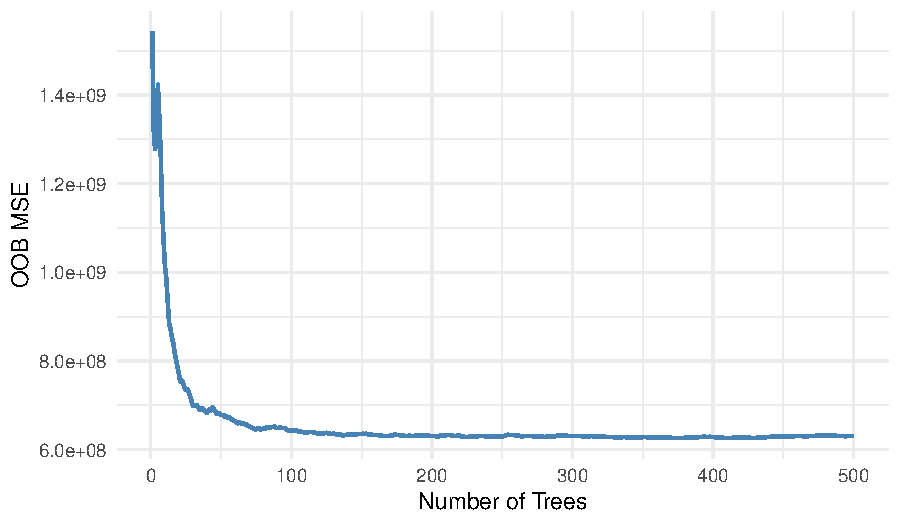
\includegraphics[keepaspectratio]{final_paper_files/figure-pdf/rf-tree-tuning-1.pdf}}

}

\caption{Out-of-bag mean squared error as a function of the number of
trees in the forest.}

\end{figure}%

Figure 1 shows how the out-of-bag MSE evolves as trees are added to the
forest. The error drops rapidly over the first 100 trees and stabilizes
near 200 trees, after which additional trees produce no meaningful
reduction in error. This pattern is consistent with the theoretical
behavior of bagged ensembles, where variance is reduced by averaging but
the benefit diminishes as more trees are added.

\subsection{Tuning the Number of Variables Per
Split}\label{tuning-the-number-of-variables-per-split}

The more meaningful hyperparameter in a random forest is \texttt{mtry},
which controls how many predictors are randomly considered as candidates
at each split. Lower values produce more decorrelated trees at the cost
of individual tree accuracy, while higher values allow each tree to
consider stronger splits but make the trees more similar to one another.
The \texttt{tuneRF} function in the \texttt{randomForest} package
searches across \texttt{mtry} values by adjusting the starting value up
and down by a chosen step factor and selecting the value that minimizes
out-of-bag error.

\begin{Shaded}
\begin{Highlighting}[]
\FunctionTok{set.seed}\NormalTok{(}\DecValTok{2026}\NormalTok{)}
\FunctionTok{tuneRF}\NormalTok{(}
  \AttributeTok{x =}\NormalTok{ train }\SpecialCharTok{|\textgreater{}} \FunctionTok{select}\NormalTok{(}\SpecialCharTok{{-}}\NormalTok{Sale\_Price),}
  \AttributeTok{y =}\NormalTok{ train}\SpecialCharTok{$}\NormalTok{Sale\_Price,}
  \AttributeTok{ntreeTry =} \DecValTok{200}\NormalTok{,}
  \AttributeTok{stepFactor =} \FloatTok{1.5}\NormalTok{,}
  \AttributeTok{improve =} \FloatTok{0.01}\NormalTok{,}
  \AttributeTok{trace =} \ConstantTok{FALSE}\NormalTok{,}
  \AttributeTok{plot =} \ConstantTok{TRUE}
\NormalTok{)}
\end{Highlighting}
\end{Shaded}

The tuning procedure tested \texttt{mtry} values of 18, 26, and 39. The
default value of 26 produced the lowest out-of-bag MSE, with the
alternatives performing less than one percent worse. This result
illustrates a well-known property of random forests, which is their
insensitivity to hyperparameter choices within a reasonable range. The
default \texttt{p/3} heuristic was confirmed to be near-optimal for this
dataset, and no additional tuning was warranted.

A final model was fit using the tuned specification. Because the
convergence analysis in the previous section showed that out-of-bag
error stabilized well before 500 trees, the final model was built with
only 200 trees to reduce computational cost while preserving essentially
identical predictive performance.

\begin{Shaded}
\begin{Highlighting}[]
\FunctionTok{set.seed}\NormalTok{(}\DecValTok{2026}\NormalTok{)}
\NormalTok{tuned\_rf\_model }\OtherTok{\textless{}{-}} \FunctionTok{randomForest}\NormalTok{(}
\NormalTok{  Sale\_Price }\SpecialCharTok{\textasciitilde{}}\NormalTok{ .,}
  \AttributeTok{data =}\NormalTok{ train,}
  \AttributeTok{ntree =} \DecValTok{200}\NormalTok{,}
  \AttributeTok{mtry =} \DecValTok{26}\NormalTok{,}
  \AttributeTok{importance =} \ConstantTok{TRUE}
\NormalTok{)}
\end{Highlighting}
\end{Shaded}

\subsection{Model Evaluation}\label{model-evaluation}

Evaluation of a random forest regression model differs meaningfully from
evaluation of a linear regression model. Because random forests make
essentially no distributional assumptions about the data or the errors,
traditional diagnostic procedures such as checking for normality of
residuals or constant variance do not apply in the same way. Instead,
evaluation focuses on direct measures of predictive performance on
held-out data and on visual inspection of where the model performs well
or poorly.

\begin{longtable}[t]{ll}
\caption{\label{tab:rf-evaluation-table}Performance metrics for the tuned random forest on held-out test data.}\\
\toprule
Metric & Value\\
\midrule
Test RMSE & \$25,154\\
Test R² & 0.911\\
OOB RMSE & \$25,127\\
\bottomrule
\end{longtable}

The test RMSE of approximately \$25,154 indicates that on average the
model predictions are off by around that amount on houses with a mean
sale price of roughly \$180,000, which corresponds to about a 14 percent
relative error. The test R² of 0.911 indicates that the model explains
91 percent of the variance in sale price on houses it was never trained
on. Perhaps most notably, the out-of-bag RMSE of \$25,127 differs from
the test RMSE by only \$27, which confirms that the out-of-bag error
provides a reliable estimate of generalization performance. This close
agreement is a practical validation of the theoretical claim that
out-of-bag estimates are nearly unbiased approximations of test error,
and it suggests that in settings where holding out a test set is
undesirable, the out-of-bag estimate alone would have produced
essentially the same conclusion about model quality. This close
alignment also serves as a robustness check on the method itself,
confirming that the training procedure produced a model that generalizes
consistently rather than one that happened to fit the training data well
by chance. For random forest regression, this kind of internal
validation is a key diagnostic tool, particularly when working with
smaller datasets where setting aside a test set would meaningfully
reduce the information available for model fitting.

\begin{figure}[H]

{\centering \pandocbounded{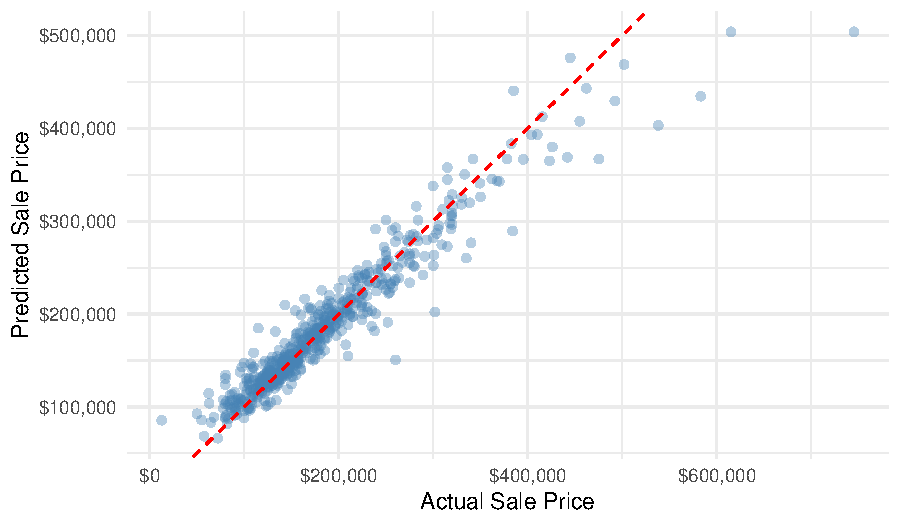
\includegraphics[keepaspectratio]{final_paper_files/figure-pdf/rf-evaluation-plot-1.pdf}}

}

\caption{Predicted versus actual sale prices on the held-out test set.
The dashed red line represents perfect prediction.}

\end{figure}%

Figure 2 plots predicted sale prices against actual sale prices on the
test set. In a well-performing model, points should cluster tightly
around the diagonal line with no systematic drift above or below it,
which would indicate that predictions are accurate across the entire
range of the response. Points cluster tightly around the diagonal
through most of the price range, with the densest region of data falling
between \$100,000 and \$300,000 where the model performs best. Two
patterns become visible at the upper end of the price range. The spread
of the points widens, indicating that prediction uncertainty grows for
more expensive homes, and the points shift systematically below the
diagonal, indicating that the model tends to underpredict the most
expensive homes. Both patterns share a common cause. Random forest
predictions are constructed by averaging responses in the terminal nodes
of each tree, which means no prediction can exceed the largest value
observed in the training data. For homes at or beyond the upper range of
the training set, the model is both less informed by data and
structurally incapable of extrapolating upward. This is a known
limitation of tree-based methods and is important to acknowledge when
applying random forests to problems where extreme values matter.

\begin{figure}[H]

{\centering \pandocbounded{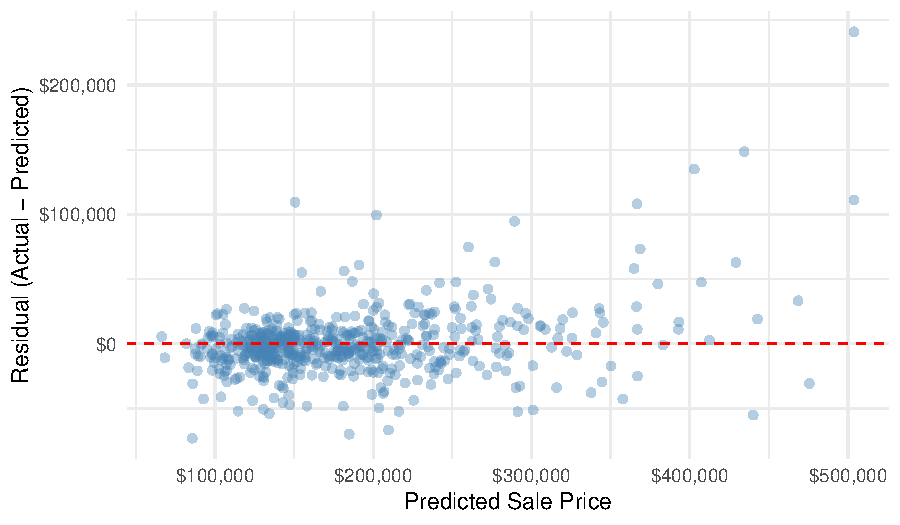
\includegraphics[keepaspectratio]{final_paper_files/figure-pdf/rf-residual-plot-1.pdf}}

}

\caption{Residuals from the tuned random forest model, defined as actual
minus predicted sale price, plotted against predicted sale price.}

\end{figure}%

The residual plot in Figure 3 makes the same patterns explicit.
Residuals fan out as predictions increase, and at the highest predicted
values the residuals are predominantly positive, which is the mirror
image of the underprediction visible in Figure 2. In a linear regression
context, this pattern would be interpreted as a violation of the
homoscedasticity assumption and would prompt remedial action such as a
log transformation of the response. In the random forest context, where
no such assumption is being made, the pattern is instead interpreted
descriptively as evidence that the model performs less reliably at the
extremes of the price distribution.

\subsection{Variable Importance}\label{variable-importance}

One of the practical advantages of random forests over linear models is
the availability of built-in variable importance measures that describe
which predictors the model is relying on most. This analysis uses
permutation-based importance, reported as percent increase in mean
squared error when a variable is permuted. The procedure takes the
out-of-bag observations and randomly shuffles the values of a single
predictor while holding all other predictors fixed, then measures how
much the out-of-bag MSE increases as a result. A variable whose
permutation causes a large increase in MSE is one the model is relying
on heavily for accurate predictions, while a variable whose permutation
changes MSE very little is one the model is effectively ignoring.

\begin{figure}[H]

{\centering \pandocbounded{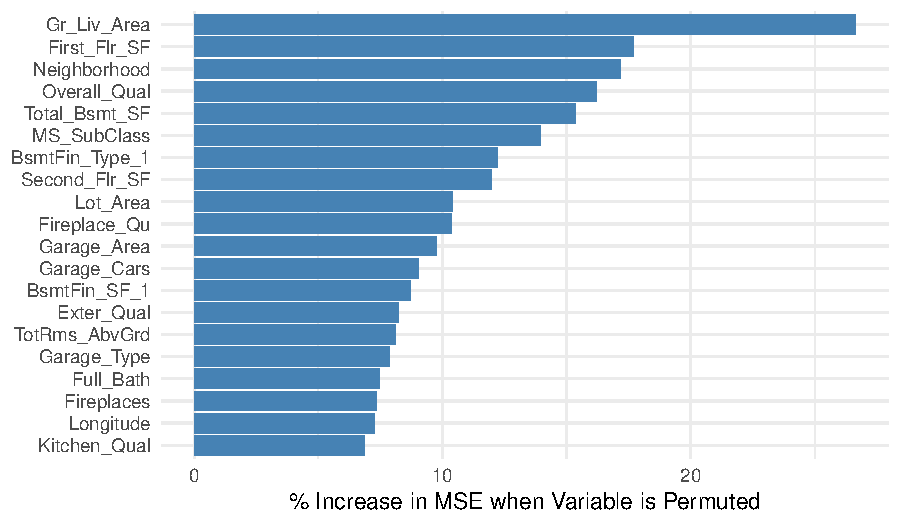
\includegraphics[keepaspectratio]{final_paper_files/figure-pdf/feature-importance-1.pdf}}

}

\caption{Top 20 predictors ranked by permutation-based variable
importance, measured as the percent increase in out-of-bag MSE when the
variable is permuted.}

\end{figure}%

Figure 4 shows the top 20 predictors ranked by permutation importance.
The most important variables are \texttt{Gr\_Liv\_Area} (above-ground
living area), followed by \texttt{First\_Flr\_SF},
\texttt{Neighborhood}, \texttt{Total\_Bsmt\_SF}, and several other size
and location variables. This ranking aligns with real-world intuition
about housing prices, where square footage and location are typically
the strongest drivers of value. The alignment between the model's most
important variables and what a domain expert would prioritize serves as
a useful sanity check that the model is learning meaningful patterns
rather than spurious ones.

Below the top 20 predictors, importance scores drop toward zero, and a
number of variables show slightly negative values. A negative percent
increase in MSE does not mean that the variable actively harms
predictions. Instead, it reflects the fact that the permutation
procedure introduces its own random variation, and when a variable
contributes essentially no predictive signal, the measured importance
fluctuates around zero and can land on either side. In practical terms,
variables at the bottom of the ranking are either carrying information
already captured by correlated predictors or have no meaningful
relationship with sale price, and the model is not relying on them
regardless.

This finding has a useful implication for model simplification. Because
many of the 80 predictors in the model contribute little to prediction,
a reduced model fit on only the top 15 to 20 predictors would likely
perform nearly as well as the full model. In settings where
interpretability, training speed, or data collection cost matter, using
variable importance to guide feature selection is a common and
defensible practice. For the purposes of this demonstration, the full
model is retained to illustrate how random forests handle
high-dimensional data without requiring that selection step.

\subsection{Summary}\label{summary}

The random forest regression model built on the Ames Housing dataset
achieves strong predictive performance on held-out test data, explaining
approximately 91 percent of the variance in sale price with a test RMSE
of about \$25,000. The close agreement between out-of-bag and test error
confirms the theoretical property that out-of-bag estimation provides a
reliable approximation of generalization error. Tuning analysis showed
that the default hyperparameters were near-optimal, consistent with the
well-known robustness of random forests to parameter choices. Variable
importance analysis produced a ranking that aligns with domain
intuition, with size and location predictors dominating the model. The
primary limitation observed was the model's tendency to underpredict the
highest-priced homes, which reflects the structural inability of
tree-based methods to extrapolate beyond the training data. Overall, the
example demonstrates that random forests are well suited to problems
with many mixed-type predictors, nonlinear relationships, and correlated
features, where linear models would require substantial preprocessing to
perform comparably. The method is most appropriate in applied settings
where predictive accuracy is the primary concern, such as price
prediction, risk scoring, ecological modeling, and medical diagnostics.
It is particularly valuable when working with datasets that contain a
large number of candidate predictors whose individual relationships with
the response are not well understood, because the algorithm can identify
informative variables without requiring the analyst to specify those
relationships in advance. The method is less appropriate when the goal
is formal statistical inference or when predictions must extend beyond
the range of the observed data, in which case a parametric model with
explicit assumptions about the relationship between predictors and the
response would be more suitable.

\section{Classification Example}\label{classification-example}

To illustrate how random forest performs in a classification setting,
this section applies the algorithm to the very well known iris dataset.
The dataset consists of 150 observations of iris flowers, each described
by a numerical feature: sepal length, sepal width, petal length, and
petal width. The response variable is the species of the flower, which
contain three classes: setosa, versicolor, and virginica. This dataset
is very useful to demonstrate the classification techniques because the
species are linearly separable but also shows some overlap, making it
simple enough to visualize yet complex enough to show the strengths of
more flexible models.

In contrast to regression, where the goal is to predict a continuous
numerical value, classification focuses on assigning observations to
categories. Random forests handle this the way you normally expects of
this model, by building multiple decision trees that each produce a
class prediction, and then is a matter of majority wins. The iris
dataset provides a clear setting to observe how random forests partition
the feature space and improve predictive accuracy compared to individual
trees, while also allowing for straightforward evaluation using metrics
such as accuracy and confusion matrices.

\subsection{Setup and Data
Preparation}\label{setup-and-data-preparation-1}

\begin{Shaded}
\begin{Highlighting}[]
\FunctionTok{library}\NormalTok{(randomForest) }
\FunctionTok{library}\NormalTok{(caret) }\SpecialCharTok{|\textgreater{}} \FunctionTok{suppressPackageStartupMessages}\NormalTok{()}
\FunctionTok{library}\NormalTok{(ggplot2)}
\FunctionTok{library}\NormalTok{(dplyr)}
\FunctionTok{library}\NormalTok{(tidyr)}
\FunctionTok{library}\NormalTok{(forcats)}
\FunctionTok{library}\NormalTok{(reprtree)}

\FunctionTok{data}\NormalTok{(iris)}

\NormalTok{trainIndex }\OtherTok{=} \FunctionTok{sample}\NormalTok{(}\DecValTok{1}\SpecialCharTok{:}\FunctionTok{nrow}\NormalTok{(iris), }\FloatTok{0.7} \SpecialCharTok{*} \FunctionTok{nrow}\NormalTok{(iris))}

\NormalTok{trainData }\OtherTok{=}\NormalTok{ iris[trainIndex, ]}
\NormalTok{testData }\OtherTok{=}\NormalTok{ iris[}\SpecialCharTok{{-}}\NormalTok{trainIndex, ]}
\end{Highlighting}
\end{Shaded}

To evaluate model performance, the data was randomly split into training
and testing sets using an 70/30 split, where 70 percent of the
observations were used to train the model and the remaining 30 percent
were held out for testing, the split was 70/30 instead of the 80/20 used
in regression because the iris dataset is significantly smaller. This
separation ensures that model performance is assessed on unseen data,
providing a more realistic measure of how well the classifier
generalizes beyond the training sample.

\subsection{Building a Model}\label{building-a-model}

\begin{verbatim}

Call:
 randomForest(formula = Species ~ ., data = trainData, type = "classification",      importance = T, proximity = T) 
               Type of random forest: classification
                     Number of trees: 500
No. of variables tried at each split: 2

        OOB estimate of  error rate: 1.9%
Confusion matrix:
           setosa versicolor virginica class.error
setosa         37          0         0  0.00000000
versicolor      0         31         1  0.03125000
virginica       0          1        35  0.02777778
\end{verbatim}

For the random forests model, some key hyperparameters to look at is
number of variables tried at each split (mtry), and number of trees
(ntree). The number of variables tried at each split being set to 2
means that for each decision tree, only two out of the four variables
are being randomly sampled as candidates. This hyperparameter matters
because this is the way of random forests to build multiple different
decision trees splits.

The model achieved an Out-of-bag (OOB) error rate of 5.71 percent,
meaning that 5.71 percent of the observation were misclassified when
each point was predicted using only the tree that did not include it
during training.

\(\frac{1}{n} \sum_{i=1}^{n} \mathbf{1}\left( y_i \neq \hat{y}_i^{\text{OOB}} \right)\)

\(\hat{y}_i^{\text{OOB}}\) =




\end{document}
